%%Énoncé
On considère un réseau téléphonique qui peut être vu comme un graphe \textit{G} dont
les sommets représentent des terminaux de commutation et les arcs représentent
des lignes de communication entre ces terminaux. Chaque arc est étiqueté par la
bande passante de la ligne qu’il représente. La bande passante d’un chemin dans
le graphe est la bande passante de son arc de bande passante minimale (autrement
dit, le maillon faible !...). On s’intéresse à l’algorithme $MaxBandWidth(G, a, b)$
qui, étant donné un réseau, représenté par un graphe \textit{G}, et deux terminaux \textit{a} et \textit{b},
renvoie la bande passante maximale d’un chemin entre \textit{a} et \textit{b}. Donnez le pseudo-code de l’algorithme $MaxBandWidth(G, a, b)$ . Piste de solution : pensez à une
variante d’un algorithme bien connu présenté dans le livre de référence.
%%Auteur
(Tanguy)\\

%%Réponse
Le pseudo-code ci-dessous est basé sur l'algorithme de Dijkstra présenté dans le livre de référence.
Á chaque arrête est associée une vitesse de bande passante en MBps correspondant à la vitesse d'échange entre les 2 sommets qu'elle relie.
Á chaque sommet est associé une vitesse de bande passante en MBps à laquelle ce sommet est joignable via le sommet $a$, cette vitesse est notée $D[u]$ avec $u \epsilon G$.
La bande passante maximale entre 2 sommets sera notée $w(a, z)$.

Au départ, la fonction $MaxBandWidth(G, a, b)$ initialise $D[v]$ à $-\infty$, noté $*$, $\forall v \epsilon G, v\neq a$ et à $0$ pour $D[a]$.
Ces valeurs sont stockées dans une file de priorité $Q$.
L'opération suivante est une boucle avec pour gardien la condition $while Q contains b$.
On retire de $Q$ l'élément qui a le $D[u]$ le plus grand. Stockons cet élément dans $u$.
Ensuite, la \textit{"relaxation procédure"} est exécutée. Elle consiste à  mettre à jour $D[z]$, $z$ étant les sommets adjacents à $u$, afin de vérifier qu'il n'existe pas un chemin possible avec une meilleure bande passante que la valeur actuelle de $D[u]$. Typiquement, $D[z] = min(D[u], w(u, z))$ si $D[z] < D[u]$.

\lstinputlisting[language=java, inputencoding=utf8]{q5.java}

Les figures ci-dessous représentent un exemple d'exécution de cet algorithme.

\begin{tabular}{ll}
   1 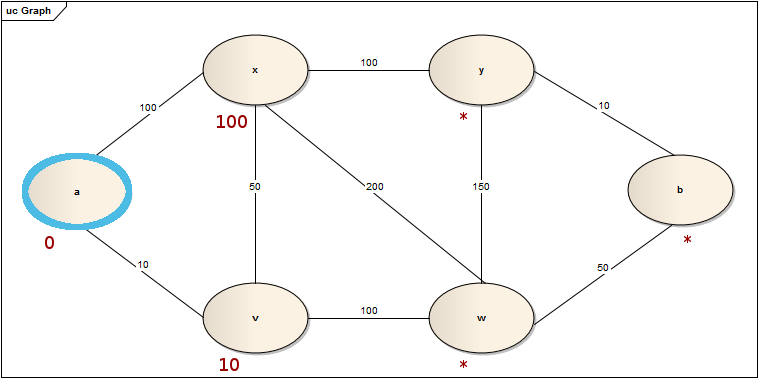
\includegraphics[width=\textwidth/2]{ea-graph/graph2-step1.png}&
   2 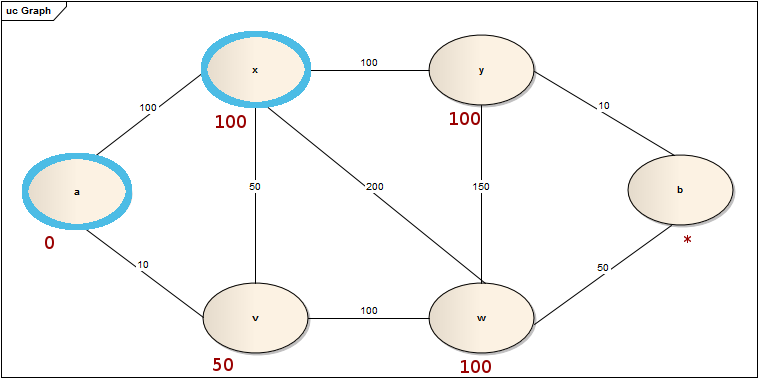
\includegraphics[width=\textwidth/2]{ea-graph/graph2-step2.png} \\
	3 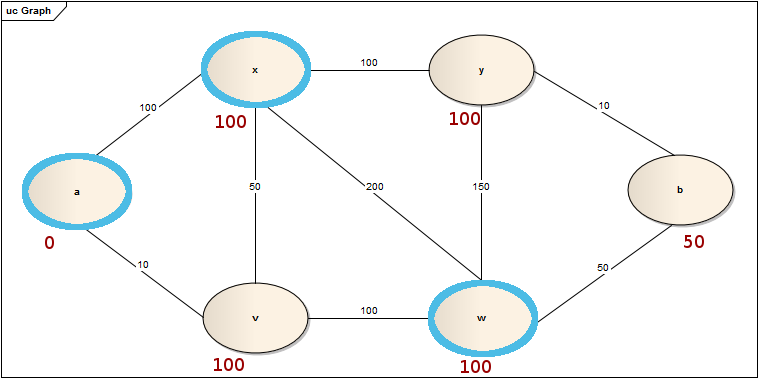
\includegraphics[width=\textwidth/2]{ea-graph/graph2-step3.png} &
	4 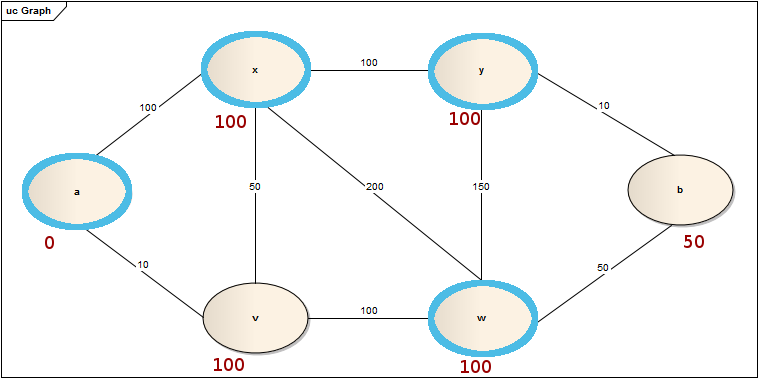
\includegraphics[width=\textwidth/2]{ea-graph/graph2-step4.png} \\
	5 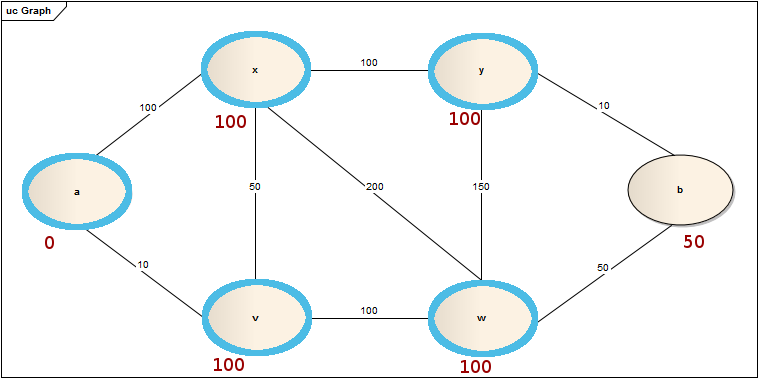
\includegraphics[width=\textwidth/2]{ea-graph/graph2-step5.png} &
	6 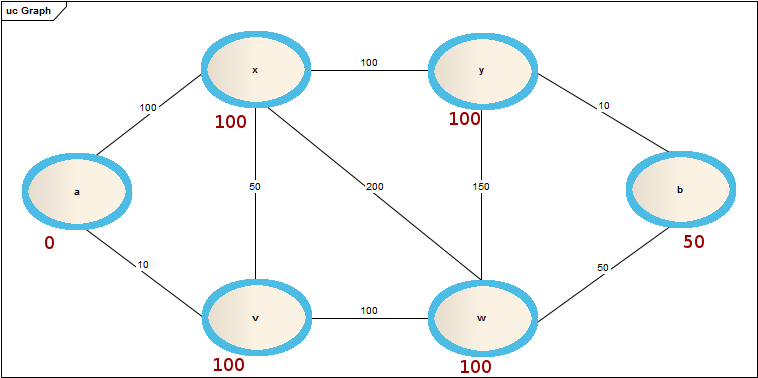
\includegraphics[width=\textwidth/2]{ea-graph/graph2-step6.png} \\
\end{tabular}

%Pré-conditions (Boris) : 
%\begin{itemize}
%	\item il n'y a pas de cycles de coûts négatifs dans le graphe \textit{G}.
%	\item[A VERIFIER!!!] Pas de poids négatifs dans G. Cette condition permet d'assurer que l'algorithme de Dijkstra fonctionne. Pourquoi ? parce qu'à chaque fois qu'un sommet est retiré de la file de priorité et ajouté à $List<D[u]>$, son label $D[u]$ est égal à $w(v,u)$, c'est à dire le chemin le plus court de $v$ à $u$.
%\end{itemize}

